% =====================================================================
% Compositions of Trigonometric Functions and Their Inverses,
% and Back Substitution
%
% Figures are generated from Asymptote sources in figures/ (see
% figures/_essayfigs.asy for the build command). The comment above each
% figure is the specification it was drawn from.
% =====================================================================

\documentclass{essay}

\usepackage{graphicx}

\DeclareMathOperator{\arcsec}{arcsec}
\DeclareMathOperator{\arccsc}{arccsc}
\DeclareMathOperator{\arccot}{arccot}
\DeclareMathOperator{\sgn}{sgn}

\title{Compositions of Trigonometric Functions and Their Inverses,\\
and Back Substitution}
\author{}
\date{}

\begin{document}

\maketitle

% ---------------------------------------------------------------------
\section{The problem}

A trigonometric function is not injective, so it has no inverse on its
natural domain. What we call $\arcsin$, $\arccos$, and the others are
inverses of \emph{restrictions}: we pick an interval on which the function
is injective and invert it there. Every subtlety in this essay comes from
that restriction.

There are three kinds of composition to understand.
\begin{enumerate}
  \item $f(f^{-1}(x))$, for example $\sin(\arcsin x)$. This is the easy
        direction.
  \item $f^{-1}(f(x))$, for example $\arcsin(\sin x)$. This equals $x$
        only on the restricted interval; elsewhere it folds $x$ back into
        that interval.
  \item $g(f^{-1}(x))$ with $g \ne f$, for example $\tan(\arcsec x)$.
        This is what back substitution in an integral asks for, and it is
        where sign errors occur.
\end{enumerate}

The single principle that resolves all of them is this: \emph{an inverse
trigonometric function returns an angle in a specific interval, and every
sign question is answered by looking at that interval.} Square roots never
carry sign information; $\sqrt{u^2} = |u|$, always.

% ---------------------------------------------------------------------
\section{Principal ranges}

\begin{definition}
The six inverse trigonometric functions used in this essay are defined as
follows. For each, $\theta = f^{-1}(x)$ is the unique $\theta$ in the stated
range with $f(\theta) = x$.
\[
\begin{array}{lll}
\text{function} & \text{domain in } x & \text{range in } \theta \\[2pt]
\hline
\arcsin x & [-1, 1] & [-\pi/2, \pi/2] \\
\arccos x & [-1, 1] & [0, \pi] \\
\arctan x & \mathbb{R} & (-\pi/2, \pi/2) \\
\arccot x & \mathbb{R} & (0, \pi) \\
\arcsec x & (-\infty, -1] \cup [1, \infty) & [0, \pi/2) \cup (\pi/2, \pi] \\
\arccsc x & (-\infty, -1] \cup [1, \infty) & [-\pi/2, 0) \cup (0, \pi/2]
\end{array}
\]
\end{definition}

The ranges are chosen to satisfy two requirements: the original function
must be injective on the range, and the range must be as close to $0$ as
possible while covering every value. Notice the pattern by quadrant.
$\arcsin$, $\arctan$, and $\arccsc$ take values in quadrants I and IV.
$\arccos$, $\arccot$, and $\arcsec$ take values in quadrants I and II. In
each case, positive $x$ gives a first-quadrant angle, and negative $x$
gives an angle in the other quadrant of the pair.

\begin{remark}
These conventions are not universal. Some texts define $\arccot$ with
range $(-\pi/2, 0) \cup (0, \pi/2]$, so that $\arccot x = \arctan(1/x)$
for $x \ne 0$. Some calculus texts define $\arcsec$ with range
$[0, \pi/2) \cup [\pi, 3\pi/2)$, chosen so that $\tan(\arcsec x) \ge 0$
always. Every formula in Section~\ref{sec:cross} depends on the convention.
Check which one your source uses before comparing answers.
\end{remark}

With the conventions above, $\arcsec$ and $\arccsc$ reduce to the more
familiar functions:
\[
\arcsec x = \arccos\frac{1}{x}, \qquad \arccsc x = \arcsin\frac{1}{x},
\qquad |x| \ge 1.
\]
Indeed, $\sec\theta = x$ if and only if $\cos\theta = 1/x$, and both
sides take values in the same interval. This identity is often the
quickest route through a computation.

% Figure description (specification used to generate figures/trig-inverse-composition-fig-ranges.pdf):
% Two unit circles side by side, each centred at the origin of its own
% coordinate axes, axes drawn through the centre and labelled $x$ and $y$
% only by small tick labels $1$ and $-1$ where the circle meets the axes.
% Left circle, titled ``$\arcsin$, $\arctan$, $\arccsc$'': draw the closed
% right half of the circle (from angle $-\pi/2$ to $\pi/2$) as a thick
% line, and the left half as a thin grey line. Mark the endpoints at
% $(0,1)$ and $(0,-1)$ with small filled dots and label them $\pi/2$ and
% $-\pi/2$. Label the region of the thick arc above the $x$-axis
% ``I'' and below the $x$-axis ``IV''. Underneath the circle, in small
% text: ``$\arcsin$: closed arc. $\arctan$: open arc, endpoints excluded.
% $\arccsc$: closed arc minus the point at angle $0$.''
% Right circle, titled ``$\arccos$, $\arccot$, $\arcsec$'': same layout,
% but the thick arc is the closed upper half (angles $0$ to $\pi$), with
% dots at $(1,0)$ labelled $0$ and $(-1,0)$ labelled $\pi$, and quadrant
% labels ``I'' and ``II''. Underneath, in small text: ``$\arccos$: closed
% arc. $\arccot$: open arc. $\arcsec$: closed arc minus the point at angle
% $\pi/2$.''
\begin{figure}[htbp]
  \centering
  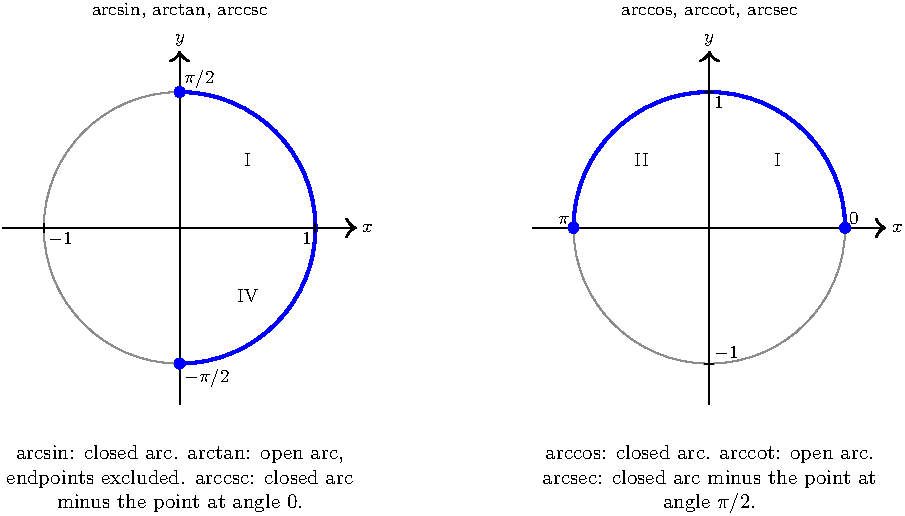
\includegraphics[width=\textwidth]{figures/trig-inverse-composition-fig-ranges.pdf}
  \caption{Principal ranges of the inverse
trigonometric functions, shown on the unit circle.}
  \label{fig:ranges}
\end{figure}

% Figure description (specification used to generate figures/trig-inverse-composition-fig-graphs.pdf):
% A $2 \times 3$ grid of six small plots, all with equal aspect ratio
% (one unit on $x$ equals one unit on $y$), each with its own axes through
% the origin, light grey dashed line $y = x$, and ticks at multiples of
% $\pi/2$ labelled $\pi/2$, $\pi$, $-\pi/2$ where they fit, plus ticks at
% $\pm 1$.
% In every plot draw the restricted function as a thin solid black curve
% and its inverse as a thick solid black curve (or the accent colour).
% Show the natural (unrestricted) function on a wider interval as a very
% light grey curve behind the restricted piece, so the reader sees which
% piece was kept.
% All panels share the window $[-4, 4]^2$, so the axes of every panel lie
% on common horizontal and vertical grid lines. Top row, left to right:
% $\arcsin$, $\arctan$, $\arcsec$; bottom row: $\arccos$, $\arccot$,
% $\arccsc$. Per panel:
% $\sin$ on $[-\pi/2, \pi/2]$ (filled endpoint dots); $\tan$ on
% $(-\pi/2, \pi/2)$ (dashed asymptotes $x = \pm\pi/2$, $y = \pm\pi/2$);
% $\sec$ on $[0, \pi/2) \cup (\pi/2, \pi]$ (asymptotes at $\pi/2$, dots at
% $(1, 0)$ and $(-1, \pi)$); $\cos$ on $[0, \pi]$ (filled endpoint dots);
% $\cot$ on $(0, \pi)$ (asymptotes at $0$ and $\pi$); $\csc$ on
% $[-\pi/2, 0) \cup (0, \pi/2]$ (asymptotes at $0$, dots at $(1, \pi/2)$
% and $(-1, -\pi/2)$).
% Each panel titled above with the name of the inverse function only,
% e.g.\ ``$\arcsec$''.
\begin{figure}[htbp]
  \centering
  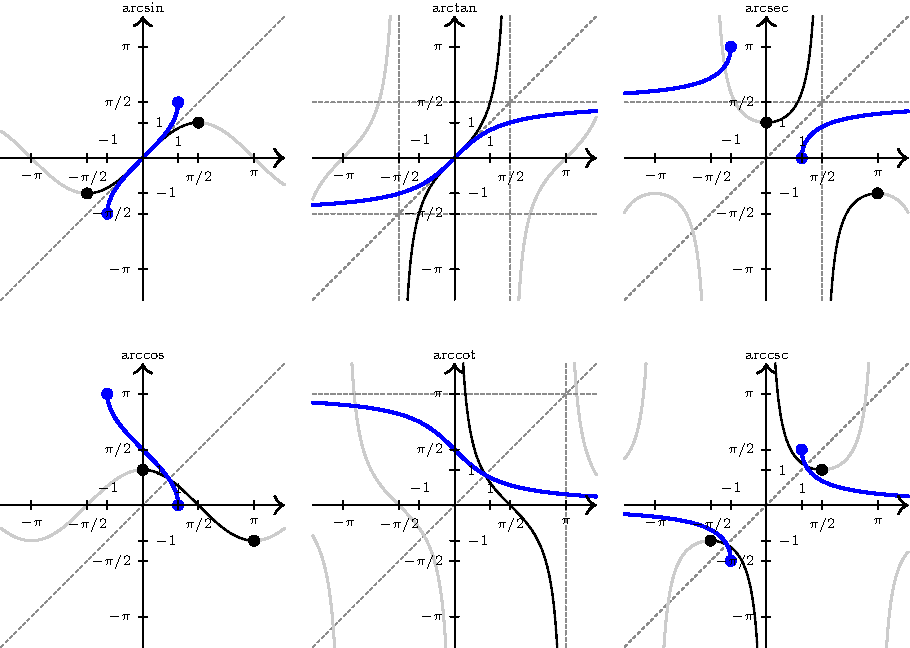
\includegraphics[width=\textwidth]{figures/trig-inverse-composition-fig-graphs.pdf}
  \caption{Restricted trigonometric functions
and their inverses. Each inverse is the reflection of the restricted
function in the line $y = x$.}
  \label{fig:graphs}
\end{figure}

% ---------------------------------------------------------------------
\section{The easy direction: $f(f^{-1}(x))$}

\begin{proposition}
For each of the six functions, $f(f^{-1}(x)) = x$ for every $x$ in the
domain of $f^{-1}$, and is undefined otherwise.
\end{proposition}

\begin{proof}
By definition $f^{-1}(x)$ is an angle $\theta$ with $f(\theta) = x$.
\end{proof}

There is nothing to compute, but the domain matters: $\sin(\arcsin 2)$ is
not $2$; it is undefined. Likewise $\sec(\arcsec \tfrac12)$ is undefined.
$\tan(\arctan x) = x$ and $\cot(\arccot x) = x$ hold for every real $x$.

% ---------------------------------------------------------------------
\section{The folding direction: $f^{-1}(f(x))$}

Here $x$ is an arbitrary angle and $f^{-1}$ must return an angle in its
range. If $x$ is already in the range, we get $x$ back. Otherwise we get
the unique angle in the range that has the same value of $f$ as $x$.
Graphically, $f^{-1}(f(x))$ is a piecewise linear function of slope
$\pm 1$.

\begin{proposition}\label{prop:fold}
For every integer $k$,
\begin{align*}
\arcsin(\sin x) &= (-1)^k (x - k\pi),
  & x &\in [k\pi - \tfrac{\pi}{2},\, k\pi + \tfrac{\pi}{2}], \\
\arccos(\cos x) &= |x - 2k\pi|,
  & x &\in [(2k-1)\pi,\, (2k+1)\pi], \\
\arctan(\tan x) &= x - k\pi,
  & x &\in (k\pi - \tfrac{\pi}{2},\, k\pi + \tfrac{\pi}{2}).
\end{align*}
\end{proposition}

\begin{proof}
In each case, check two things: the right-hand side lies in the range of
the inverse function, and $f$ of the right-hand side equals $f(x)$.

For $\arcsin$: if $x \in [k\pi - \pi/2, k\pi + \pi/2]$ then
$x - k\pi \in [-\pi/2, \pi/2]$, and so is its negative. Also
$\sin((-1)^k(x - k\pi)) = (-1)^k \sin(x - k\pi) = (-1)^k(-1)^k \sin x
= \sin x$, using $\sin(x - k\pi) = (-1)^k \sin x$ and the oddness of
$\sin$.

For $\arccos$: if $x \in [(2k-1)\pi, (2k+1)\pi]$ then
$x - 2k\pi \in [-\pi, \pi]$, so $|x - 2k\pi| \in [0, \pi]$. Since
$\cos$ is even and $2\pi$-periodic,
$\cos|x - 2k\pi| = \cos(x - 2k\pi) = \cos x$.

For $\arctan$: $x - k\pi \in (-\pi/2, \pi/2)$, and $\tan$ has period
$\pi$.
\end{proof}

\begin{example}
$\arcsin(\sin 3)$. Since $3 \in [\pi/2, 3\pi/2]$, take $k = 1$:
the result is $-(3 - \pi) = \pi - 3 \approx 0.14$. Check: $\pi - 3$ lies
in $[-\pi/2, \pi/2]$, and $\sin(\pi - 3) = \sin 3$.
\end{example}

\begin{example}
$\arccos(\cos(-1)) = 1$, because $\cos$ is even and $1 \in [0, \pi]$.
Note that $\arcsin(\sin(-1)) = -1$. The two folds differ because the
ranges differ.
\end{example}

\begin{example}
$\arctan(\tan 2) = 2 - \pi$, since $2 \in (\pi/2, 3\pi/2)$.
\end{example}

% Figure description (specification used to generate figures/trig-inverse-composition-fig-fold.pdf):
% Three plots stacked vertically, each full text width and about 4 cm
% tall, sharing the same horizontal axis range $x \in [-2\pi, 2\pi]$ with
% ticks at every multiple of $\pi/2$, labelled $-2\pi, -3\pi/2, \dots,
% 2\pi$. Equal scaling on both axes within each plot.
% Top plot: $y = \arcsin(\sin x)$. A triangle wave with slope $\pm 1$,
% peaks at $x = \pi/2 + 2k\pi$ with $y = \pi/2$, troughs at
% $x = -\pi/2 + 2k\pi$ with $y = -\pi/2$. Horizontal dashed grey lines at
% $y = \pm\pi/2$, labelled at the left. The segment over
% $[-\pi/2, \pi/2]$ (the principal range, where the graph coincides with
% $y = x$) is drawn thick or in the accent colour; the rest thin. Also
% draw the line $y = x$ as a light grey dashed line over the whole range
% for comparison. Mark the point $(3, \pi - 3)$ with a small dot and label
% ``$\arcsin(\sin 3) = \pi - 3$''.
% Middle plot: $y = \arccos(\cos x)$. A triangle wave with values in
% $[0, \pi]$: zeros at $x = 2k\pi$, peaks $y = \pi$ at
% $x = (2k+1)\pi$. Dashed grey lines at $y = 0$ and $y = \pi$. Thick
% segment over $[0, \pi]$. Light grey dashed $y = x$. Mark the point
% $(-1, 1)$ with a dot labelled ``$\arccos(\cos(-1)) = 1$''.
% Bottom plot: $y = \arctan(\tan x)$. A sawtooth: lines of slope 1 on
% each interval $(k\pi - \pi/2, k\pi + \pi/2)$, open circles at the jump
% endpoints $y = \pm\pi/2$, and dashed vertical grey lines at
% $x = \pi/2 + k\pi$ where $\tan$ is undefined. Thick segment over
% $(-\pi/2, \pi/2)$. Light grey dashed $y = x$. Mark the point
% $(2, 2 - \pi)$ with a dot labelled ``$\arctan(\tan 2) = 2 - \pi$''.
% Each plot has its formula as a small title at the top left.
\begin{figure}[htbp]
  \centering
  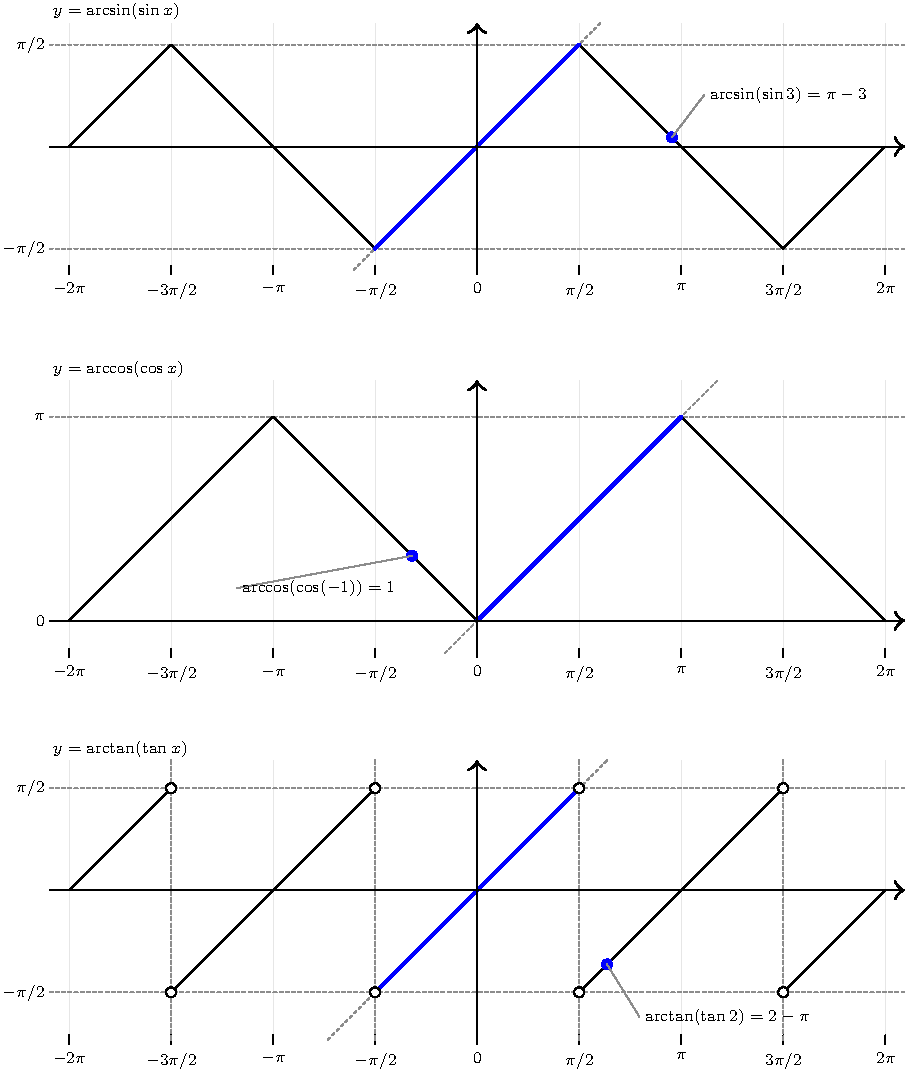
\includegraphics[width=\textwidth]{figures/trig-inverse-composition-fig-fold.pdf}
  \caption{The folding compositions on
$[-2\pi, 2\pi]$. Each graph is the identity on the principal range,
shown thick, and is folded back into the range elsewhere.}
  \label{fig:fold}
\end{figure}

% ---------------------------------------------------------------------
\section{Cross compositions: $g(f^{-1}(x))$}\label{sec:cross}

This is the case that matters for integration. We know one trigonometric
value of an angle, $f(\theta) = x$, and the interval containing $\theta$.
We want a different trigonometric value $g(\theta)$ as an algebraic
expression in $x$.

\subsection{The method}

\begin{enumerate}
  \item Set $\theta = f^{-1}(x)$. Write down what you know: $f(\theta) = x$
        and the interval containing $\theta$.
  \item Use a Pythagorean identity,
        \[
        \sin^2\theta + \cos^2\theta = 1, \qquad
        1 + \tan^2\theta = \sec^2\theta, \qquad
        1 + \cot^2\theta = \csc^2\theta,
        \]
        to find $g(\theta)^2$, or the square of some function from which
        $g(\theta)$ follows without a further square root.
  \item Determine the sign of $g(\theta)$ on the interval. If it is
        constant, take the root with that sign. If it is not constant,
        the sign depends on which part of the range $\theta$ lies in,
        which in turn depends on the sign of $x$; express it through $x$.
  \item Simplify with $\sqrt{x^2} = |x|$, never $\sqrt{x^2} = x$.
  \item Check the domain: exclude $x$ for which $g(\theta)$ is undefined.
\end{enumerate}

Step 3 is the whole content of the method. It is cheap to carry out, and
skipping it is what produces wrong answers.

\subsection{A worked case where the sign is constant}

\begin{example}
Consider $\csc(\arcsec x)$. Let $\theta = \arcsec x$. Then
$\cos\theta = 1/x$ and $\theta \in [0, \pi/2) \cup (\pi/2, \pi]$, so
\[
\sin^2\theta = 1 - \frac{1}{x^2} = \frac{x^2 - 1}{x^2}.
\]
On $[0, \pi]$ we have $\sin\theta \ge 0$, on both parts of the range.
Therefore
\[
\sin\theta = \frac{\sqrt{x^2 - 1}}{\sqrt{x^2}}
           = \frac{\sqrt{x^2 - 1}}{|x|},
\qquad
\csc(\arcsec x) = \frac{|x|}{\sqrt{x^2 - 1}},
\qquad |x| > 1.
\]
The points $x = \pm 1$ are excluded because there $\theta \in \{0, \pi\}$
and $\sin\theta = 0$.
\end{example}

The absolute value appears because $\sin\theta$ keeps its sign across the
range while $x = \sec\theta$ changes sign. A formula written in terms of
$x$ alone must undo that sign change.

% Figure description (specification used to generate figures/trig-inverse-composition-fig-cscsign.pdf):
% Two panels stacked on a shared horizontal axis $\theta \in [0, \pi]$ (ticks
% at multiples of $\pi/4$, a dashed vertical asymptote at $\pi/2$). Top panel:
% $x = \sec\theta$ as a thick curve, blue on $[0, \pi/2)$ (above $x = 1$) and
% gray on $(\pi/2, \pi]$ (below $x = -1$), with filled dots at $(0, 1)$ and
% $(\pi, -1)$, dotted lines at $x = \pm 1$, and the regions between the curve
% and the axis tinted to match. Bottom panel: $\sin\theta$ on $[0, \pi]$,
% with the same blue and gray halves and the same tints under the curve,
% always above the axis. Each panel carries a short label.
\begin{figure}[htbp]
  \centering
  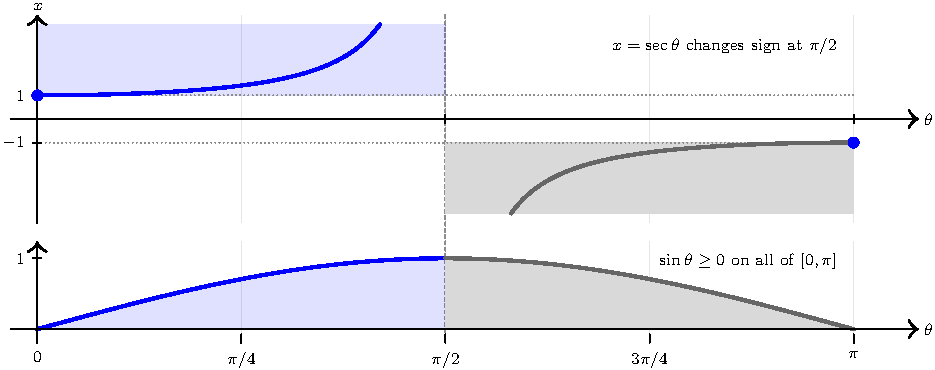
\includegraphics[width=\textwidth]{figures/trig-inverse-composition-fig-cscsign.pdf}
  \caption{On the range of $\arcsec$, $x = \sec\theta$ changes sign at
$\pi/2$ (top) while $\sin\theta$ stays nonnegative (bottom). The two halves
of the range are shown in the same colours in both panels.}
  \label{fig:cscsign}
\end{figure}

\subsection{A worked case where the sign changes}

\begin{example}
$\tan(\arcsec x)$. With $\theta$ as before,
$\tan^2\theta = \sec^2\theta - 1 = x^2 - 1$. Now $\tan\theta \ge 0$ on
$[0, \pi/2)$, which is the case $x \ge 1$, and $\tan\theta \le 0$ on
$(\pi/2, \pi]$, which is the case $x \le -1$. So
\[
\tan(\arcsec x) =
\begin{cases}
  \phantom{-}\sqrt{x^2 - 1}, & x \ge 1, \\
  -\sqrt{x^2 - 1}, & x \le -1,
\end{cases}
\]
that is, $\tan(\arcsec x) = \sgn(x)\sqrt{x^2 - 1}$ (see Figure~\ref{fig:secant-sign}, where the sign of $\tan\theta$ matches the sign of $x$ on each part of the range).
Alternatively, $\tan\theta = \sin\theta / \cos\theta
= \dfrac{\sqrt{x^2-1}}{|x|} \cdot x$, which gives the same result, since
$x / |x| = \sgn x$. Computing a sign-stable function first and deriving
the others from it is often the cleanest route.
\end{example}

% Copy of the figure in Section~\ref{sec:cross}'s secant-substitution
% subsection (same PDF, same specification as fig:secant below), repeated
% here so the example can refer to it.
\begin{figure}[htbp]
  \centering
  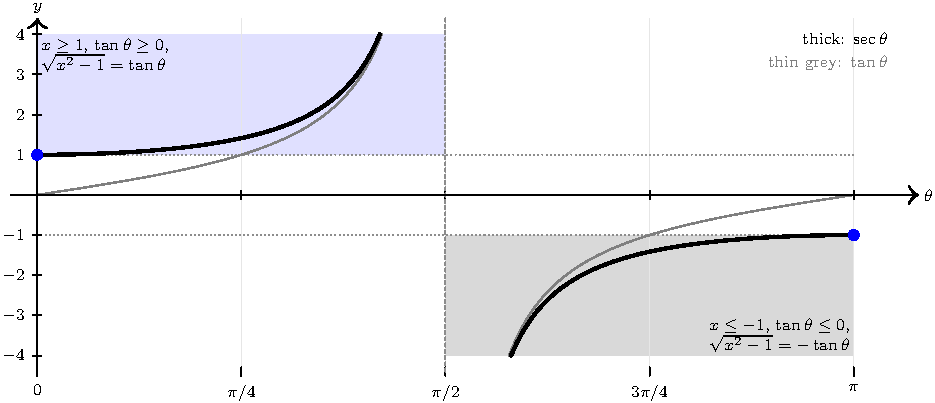
\includegraphics[width=\textwidth]{figures/trig-inverse-composition-fig-secant.pdf}
  \caption{For $\theta = \arcsec x$, the sign of $\tan\theta$ equals the
sign of $x$: both are nonnegative on $[0, \pi/2)$ and both are nonpositive
on $(\pi/2, \pi]$.}
  \label{fig:secant-sign}
\end{figure}

\subsection{A uniform tool: the signed reference point}

The familiar reference-triangle method draws a right triangle with acute
angle $\theta$ and reads off side lengths. It is correct only when
$\theta \in (0, \pi/2)$, that is, only for positive $x$ in most cases.
For the other half of the range it silently gives the wrong sign.

The correct generalisation replaces the triangle with a point $(X, Y)$ on
the terminal side of $\theta$, at distance $r = \sqrt{X^2 + Y^2} > 0$
from the origin. Then
\[
\begin{gathered}
\sin\theta = \frac{Y}{r},\quad
\cos\theta = \frac{X}{r},\quad
\tan\theta = \frac{Y}{X},\\
\csc\theta = \frac{r}{Y},\quad
\sec\theta = \frac{r}{X},\quad
\cot\theta = \frac{X}{Y}.
\end{gathered}
\]
Here $X$ and $Y$ are signed coordinates, and the quadrant of $\theta$
dictates their signs. To evaluate $g(f^{-1}(x))$:
\begin{enumerate}
  \item Choose $X$, $Y$, $r$ consistent with $f(\theta) = x$, keeping
        $r > 0$.
  \item Fix the sign of the remaining coordinate from the range of
        $f^{-1}$.
  \item Read off $g(\theta)$.
\end{enumerate}

\begin{example}
$\theta = \arcsec x$, so $r / X = x$. Since $r > 0$, $X$ has the sign of
$x$; take $X = \sgn x$ and $r = |x|$. Then
$Y^2 = r^2 - X^2 = x^2 - 1$, and since $\theta \in [0, \pi]$, $Y \ge 0$,
so $Y = \sqrt{x^2 - 1}$. Every value follows at once:
\[
\sin\theta = \frac{\sqrt{x^2-1}}{|x|},\quad
\tan\theta = \frac{\sqrt{x^2-1}}{\sgn x} = \sgn(x)\sqrt{x^2-1},
\]
\[
\csc\theta = \frac{|x|}{\sqrt{x^2-1}},\quad
\cot\theta = \frac{\sgn x}{\sqrt{x^2-1}}.
\]
\end{example}

% Figure description (specification used to generate figures/trig-inverse-composition-fig-refpoint.pdf):
% Two panels side by side, each with coordinate axes through the origin
% and equal scaling, window $x \in [-2.5, 2.5]$, $y \in [-0.5, 2.5]$,
% with a light grey circle of radius 2 centred at the origin.
% Left panel, titled ``$x = 2$: $\theta = \pi/3$''. Draw the ray from the
% origin at angle $\pi/3$ to the point $P = (1, \sqrt{3})$, marked with a
% dot and labelled ``$(X, Y) = (1, \sqrt{3})$''. Draw a dashed vertical
% segment from $P$ down to $(1, 0)$, forming a right triangle with the
% $x$-axis. Label the hypotenuse ``$r = 2$'', the horizontal leg
% ``$X = 1$'', the vertical leg ``$Y = \sqrt{3}$''. Draw an arc at the
% origin from the positive $x$-axis to the ray, labelled $\theta$. Below
% the panel: ``$\tan\theta = Y/X = \sqrt{3} > 0$''.
% Right panel, titled ``$x = -2$: $\theta = 2\pi/3$''. Draw the ray at
% angle $2\pi/3$ to $P = (-1, \sqrt{3})$, dot labelled
% ``$(X, Y) = (-1, \sqrt{3})$''. Dashed vertical segment from $P$ to
% $(-1, 0)$. Label the hypotenuse ``$r = 2$'', the horizontal leg
% ``$X = -1$'' (emphasise the minus sign, e.g.\ in the accent colour),
% vertical leg ``$Y = \sqrt{3}$''. Arc from the positive $x$-axis
% counterclockwise to the ray labelled $\theta$. Below the panel:
% ``$\tan\theta = Y/X = -\sqrt{3} < 0$''.
% Additionally, in the right panel, draw faintly in grey the mirror-image
% first-quadrant triangle (the ``naive'' reference triangle, as in the left
% panel) with a small grey label ``naive triangle: would give
% $+\sqrt{3}$''.
\begin{figure}[htbp]
  \centering
  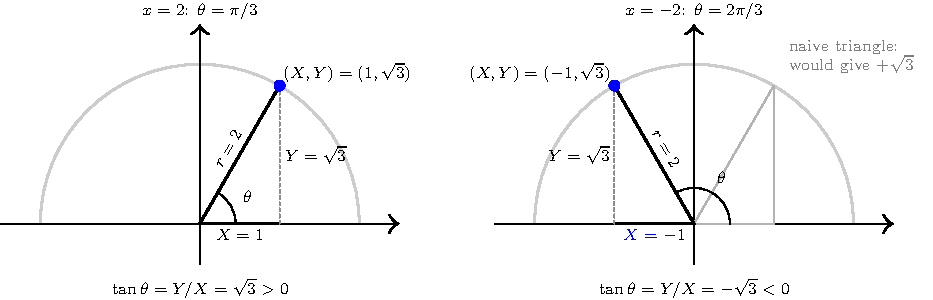
\includegraphics[width=\textwidth]{figures/trig-inverse-composition-fig-refpoint.pdf}
  \caption{The reference triangle versus
the signed reference point for $\theta = \arcsec x$. For $x = -2$ the
angle is in quadrant II, and the triangle picture, which assumes an acute
angle, gives the wrong sign for $\tan\theta$.}
  \label{fig:refpoint}
\end{figure}

\subsection{Table of cross compositions}

The following table collects the common cases under the conventions of
Section~2. The last column states where the sign of the result comes from.
{\small
\renewcommand{\arraystretch}{1.6}
\[
\begin{array}{llll}
\text{expression} & \text{value} & \text{valid for} & \text{sign source} \\
\hline
\sin(\arccos x) & \sqrt{1 - x^2} & |x| \le 1 & \sin \ge 0,\ [0,\pi] \\
\cos(\arcsin x) & \sqrt{1 - x^2} & |x| \le 1 & \cos \ge 0,\ [-\tfrac{\pi}{2},\tfrac{\pi}{2}] \\
\tan(\arcsin x) & \dfrac{x}{\sqrt{1 - x^2}} & |x| < 1 & \sgn\sin\theta = \sgn x \\
\tan(\arccos x) & \dfrac{\sqrt{1 - x^2}}{x} & 0 < |x| \le 1 & \sgn\cos\theta = \sgn x \\
\sin(\arctan x) & \dfrac{x}{\sqrt{1 + x^2}} & \mathbb{R} & \cos > 0,\ (-\tfrac{\pi}{2},\tfrac{\pi}{2}) \\
\cos(\arctan x) & \dfrac{1}{\sqrt{1 + x^2}} & \mathbb{R} & \text{same} \\
\sin(\arccot x) & \dfrac{1}{\sqrt{1 + x^2}} & \mathbb{R} & \sin > 0,\ (0,\pi) \\
\cos(\arccot x) & \dfrac{x}{\sqrt{1 + x^2}} & \mathbb{R} & \text{same} \\
\sin(\arcsec x) & \dfrac{\sqrt{x^2 - 1}}{|x|} & |x| \ge 1 & \sin \ge 0,\ [0,\pi] \\
\tan(\arcsec x) & \sgn(x)\sqrt{x^2 - 1} & |x| \ge 1 & \text{branch-dependent} \\
\csc(\arcsec x) & \dfrac{|x|}{\sqrt{x^2 - 1}} & |x| > 1 & \sin \ge 0,\ [0,\pi] \\
\cos(\arccsc x) & \dfrac{\sqrt{x^2 - 1}}{|x|} & |x| \ge 1 & \cos \ge 0,\ [-\tfrac{\pi}{2},\tfrac{\pi}{2}] \\
\cot(\arccsc x) & \sgn(x)\sqrt{x^2 - 1} & |x| \ge 1 & \text{branch-dependent}
\end{array}
\]
}

A pattern is visible. In every row, the result has the form
$\pm\sqrt{\cdot}$ times a power of $x$ or $|x|$. Whether $x$ or $|x|$
appears is decided by whether the target function changes sign across
the range of the inverse function. Memorising the table is unnecessary;
rederiving any row takes three lines once the range is known.

% ---------------------------------------------------------------------
\section{Back substitution in integrals}

In a trigonometric substitution we set $x = a\,f(\theta)$, integrate in
$\theta$, and obtain an answer containing trigonometric functions of
$\theta$. To return to $x$ we must evaluate expressions such as
$\sin\theta$ or $\tan\theta$ with $\theta = f^{-1}(x/a)$. That is exactly
a cross composition, and everything in Section~\ref{sec:cross} applies.

For the substitution to be legitimate, $x = a f(\theta)$ must be
invertible on the interval of integration, so $\theta$ really is
$f^{-1}(x/a)$ there. This is what fixes the interval for $\theta$; it is
not a matter of choice once the inverse function's convention is set.

\subsection{Substitutions without sign trouble}

For $x = a\sin\theta$ with $\theta \in [-\pi/2, \pi/2]$, and for
$x = a\tan\theta$ with $\theta \in (-\pi/2, \pi/2)$, the radical becomes
$a\cos\theta$ or $a\sec\theta$, both nonnegative on the whole interval.
One interval covers the entire domain in $x$, and no case split arises.

\begin{example}
$\displaystyle\int \sqrt{1 - x^2}\,dx$. Put $x = \sin\theta$,
$\theta \in [-\pi/2, \pi/2]$, so $\sqrt{1 - x^2} = \cos\theta$ and
$dx = \cos\theta\,d\theta$:
\[
\int \cos^2\theta\,d\theta
= \frac{\theta + \sin\theta\cos\theta}{2} + C.
\]
Back substitution: $\theta = \arcsin x$, $\sin\theta = x$, and
$\cos\theta = \cos(\arcsin x) = \sqrt{1 - x^2}$ from the table. Hence
\[
\int \sqrt{1 - x^2}\,dx = \frac{\arcsin x + x\sqrt{1 - x^2}}{2} + C,
\qquad |x| \le 1.
\]
Note that the double-angle form $\tfrac14 \sin 2\theta$ must be expanded
to $\tfrac12\sin\theta\cos\theta$ before back substituting. Writing
$\sin(2\arcsin x)$ is correct but not algebraic.
\end{example}

\begin{example}
$\displaystyle\int \frac{dx}{x^2\sqrt{x^2 + 4}}$. Put $x = 2\tan\theta$,
$\theta \in (-\pi/2, \pi/2)$, $\theta \ne 0$. Then
$\sqrt{x^2 + 4} = 2\sec\theta$ and $dx = 2\sec^2\theta\,d\theta$:
\[
\int \frac{2\sec^2\theta}{4\tan^2\theta \cdot 2\sec\theta}\,d\theta
= \frac14 \int \frac{\cos\theta}{\sin^2\theta}\,d\theta
= -\frac{1}{4\sin\theta} + C.
\]
Back substitution: $\sin\theta = \sin(\arctan(x/2)) = \dfrac{x/2}{\sqrt{1
+ x^2/4}} = \dfrac{x}{\sqrt{x^2 + 4}}$. Hence
\[
\int \frac{dx}{x^2\sqrt{x^2 + 4}} = -\frac{\sqrt{x^2 + 4}}{4x} + C.
\]
The formula for $\sin(\arctan u)$ carries the sign of $u$ on its own, so
the result is correct for negative $x$ without any case analysis.
\end{example}

\subsection{The secant substitution}

For $\sqrt{x^2 - a^2}$ the domain $|x| \ge a$ has two components, and no
single interval for $\theta$ covers both while keeping $\tan\theta$ of
one sign. With $x = a\sec\theta$:
\[
\sqrt{x^2 - a^2} = a|\tan\theta| =
\begin{cases}
  \phantom{-}a\tan\theta, & x \ge a,\ \theta \in [0, \pi/2), \\
  -a\tan\theta, & x \le -a,\ \theta \in (\pi/2, \pi].
\end{cases}
\]
Work each branch separately, then combine.

\begin{example}\label{ex:secant}
$\displaystyle\int \frac{\sqrt{x^2 - 1}}{x}\,dx$. Put $x = \sec\theta$,
$dx = \sec\theta\tan\theta\,d\theta$.

\emph{Branch $x \ge 1$.} $\sqrt{x^2 - 1} = \tan\theta$, and
\[
\int \frac{\tan\theta}{\sec\theta}\,\sec\theta\tan\theta\,d\theta
= \int \tan^2\theta\,d\theta
= \tan\theta - \theta + C.
\]
Back substitution: $\tan\theta = \sqrt{x^2 - 1}$, giving
$\sqrt{x^2 - 1} - \arcsec x + C$.

\emph{Branch $x \le -1$.} $\sqrt{x^2 - 1} = -\tan\theta$, so the
integrand becomes $-\tan^2\theta$ and the antiderivative is
$-\tan\theta + \theta + C$. Back substitution: here
$\tan\theta = -\sqrt{x^2 - 1}$, so $-\tan\theta = \sqrt{x^2 - 1}$, giving
$\sqrt{x^2 - 1} + \arcsec x + C$.

\emph{Check} by differentiation, using
$\dfrac{d}{dx}\arcsec x = \dfrac{1}{|x|\sqrt{x^2 - 1}}$. For $x < -1$,
$|x| = -x$, and
\[
\frac{d}{dx}\left(\sqrt{x^2 - 1} + \arcsec x\right)
= \frac{x}{\sqrt{x^2 - 1}} - \frac{1}{x\sqrt{x^2 - 1}}
= \frac{x^2 - 1}{x\sqrt{x^2 - 1}}
= \frac{\sqrt{x^2 - 1}}{x}.
\]

\emph{Combining.} Since $\arcsec(-u) = \pi - \arcsec u$, on $x \le -1$
we have $\arcsec x = \pi - \arcsec|x|$, so the second branch equals
$\sqrt{x^2 - 1} - \arcsec|x|$ up to a constant. A single formula valid on
both components is
\[
\int \frac{\sqrt{x^2 - 1}}{x}\,dx
= \sqrt{x^2 - 1} - \arcsec|x| + C.
\]
Since $\arcsec|x| = \arctan\sqrt{x^2 - 1}$ for $|x| \ge 1$, this can also
be written $\sqrt{x^2 - 1} - \arctan\sqrt{x^2 - 1} + C$, which avoids
$\arcsec$ altogether. (Strictly, the constant may differ on the two
components, as with any antiderivative on a disconnected domain.)
\end{example}

\begin{remark}
Had we used the acute reference triangle on the second branch, we would
have written $\tan\theta = \sqrt{x^2 - 1}$ and obtained
$-\sqrt{x^2 - 1} + \arcsec x$, whose derivative is the negative of the
integrand for $x < -1$. The error is invisible unless one differentiates
on the negative branch.
\end{remark}

% Figure description (specification used to generate figures/trig-inverse-composition-fig-secant.pdf):
% A single plot with horizontal axis $\theta \in [0, \pi]$ (ticks at $0$,
% $\pi/4$, $\pi/2$, $3\pi/4$, $\pi$) and vertical axis from $-4$ to $4$.
% Draw $y = \sec\theta$ as a thick black curve with a dashed vertical
% asymptote at $\theta = \pi/2$: on $[0, \pi/2)$ it rises from $1$ to
% $+\infty$; on $(\pi/2, \pi]$ it rises from $-\infty$ to $-1$.
% Draw $y = \tan\theta$ as a thin grey curve on the same axes, using the
% same asymptote.
% Shade lightly the region of the plane above $y = 1$ over
% $\theta \in [0, \pi/2)$ and label it ``$x \ge 1$, $\tan\theta \ge 0$,
% $\sqrt{x^2-1} = \tan\theta$''. Shade lightly (a different light tone or
% hatching) the region below $y = -1$ over $\theta \in (\pi/2, \pi]$ and
% label it ``$x \le -1$, $\tan\theta \le 0$, $\sqrt{x^2-1} = -\tan\theta$''.
% Mark the points $(0, 1)$ and $(\pi, -1)$ with filled dots. Draw thin
% dotted horizontal lines at $y = 1$ and $y = -1$. Legend at upper right:
% ``thick: $\sec\theta$'', ``thin grey: $\tan\theta$''.
\begin{figure}[htbp]
  \centering
  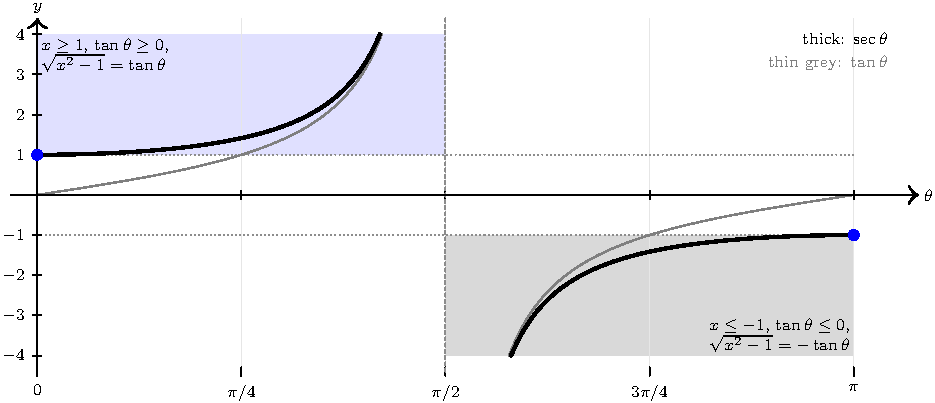
\includegraphics[width=\textwidth]{figures/trig-inverse-composition-fig-secant.pdf}
  \caption{The substitution $x = \sec\theta$
maps the two parts of the $\theta$-range onto the two components of the
$x$-domain. The sign of $\tan\theta$, and hence the relation between
$\sqrt{x^2-1}$ and $\tan\theta$, differs on the two parts.}
  \label{fig:secant}
\end{figure}

\subsection{Definite integrals: change the limits instead}

For a definite integral one can avoid back substitution entirely by
converting the limits to $\theta$. The branch issue does not disappear,
but it becomes explicit: the limits tell you which part of the range you
are in.

\begin{example}
$\displaystyle\int_{-2}^{-\sqrt{2}} \frac{dx}{x\sqrt{x^2 - 1}}$. The
whole interval lies in $x \le -1$, so with $x = \sec\theta$ we have
$\theta \in (\pi/2, \pi]$ and $\sqrt{x^2 - 1} = -\tan\theta$. The
integrand becomes
\[
\frac{\sec\theta\tan\theta}{\sec\theta\cdot(-\tan\theta)}\,d\theta
= -\,d\theta.
\]
The limits are $\arcsec(-2) = 2\pi/3$ and $\arcsec(-\sqrt{2}) = 3\pi/4$.
Hence
\[
\int_{-2}^{-\sqrt{2}} \frac{dx}{x\sqrt{x^2 - 1}}
= -\left(\frac{3\pi}{4} - \frac{2\pi}{3}\right) = -\frac{\pi}{12}.
\]
Sanity check: on $[-2, -\sqrt{2}]$ the integrand is negative (negative
numerator sign from $x$, positive radical) and the interval is traversed
left to right, so the integral must be negative. Ignoring the sign of
$\tan\theta$ would have produced $+\pi/12$.
\end{example}

% ---------------------------------------------------------------------
\section{Summary}

The inverse trigonometric functions are inverses of restrictions, and
every composition is governed by the restricted interval.
$f(f^{-1}(x)) = x$ on the domain of $f^{-1}$. $f^{-1}(f(x))$ folds $x$
into the range of $f^{-1}$ and equals $x$ only there. A cross composition
$g(f^{-1}(x))$ is computed with a Pythagorean identity, and its sign is
read from the range of $f^{-1}$, not from a square root and not from an
acute triangle. When $g$ keeps its sign across the range while $x$ does
not, an absolute value appears; when $g$ changes sign with $x$, the
result carries the sign of $x$.

Back substitution is the same computation. For sine and tangent
substitutions the relevant signs are constant and nothing goes wrong. For
secant and cosecant substitutions the $x$-domain splits in two, the
$\theta$-range splits accordingly, and each branch must be handled on its
own before the answers are combined. The reliable check is to
differentiate the result on each branch separately.

% ---------------------------------------------------------------------
\section{Self-check questions}

\begin{enumerate}
  \item Why must a trigonometric function be restricted before it has an
        inverse? For which $x$ is $f(f^{-1}(x))=x$ defined?
  \item Explain why $\arcsin(\sin x)$ need not equal $x$. Find
        $\arcsin(\sin(5\pi/6))$ and $\arccos(\cos(5\pi/3))$, checking
        that each answer lies in the appropriate principal range.
  \item What happens at $x=\pi/2$ in $\arctan(\tan x)$? Why does this
        composition have jumps, whereas $\arcsin(\sin x)$ does not?
  \item What is $\sqrt{x^2}$ for arbitrary real $x$? Under what
        condition may you replace it by $x$? Explain how this matters
        when a Pythagorean identity is used to find a trigonometric
        function of an inverse angle.
  \item Derive $\tan(\arccos x)$ from an identity and the range of
        $\arccos$. State its domain, including any points where the
        composition is undefined.
  \item Derive $\cos(\arccsc x)$ for both signs of $x$. Explain where
        the absolute value in the denominator comes from, and check
        the endpoints of the domain.
  \item Compare the signs of $\cos(\arccsc x)$ and
        $\cot(\arccsc x)$ for $x>1$ and $x<-1$. Derive the latter
        expression and explain when $|x|$ or $\sgn(x)$ enters each
        formula.
  \item Let $\theta=\arcsec x$. Choose a signed reference point for
        $\theta$ when $x=-2$, and use it to find $\sin\theta$ and
        $\tan\theta$. Which sign would an acute reference triangle get
        wrong?
  \item A student proposes
        $\sin(\arcsec x)=\sqrt{x^2-1}/x$ and
        $\tan(\arcsec x)=\sqrt{x^2-1}$ for $|x|\ge1$. Test both at
        $x=-2$, correct any errors, and explain from the principal
        range why one correction uses $|x|$ and the other uses
        $\sgn(x)$.
  \item For $a>0$ and $x=a\sec\theta$ on the principal range of
        $\arcsec$, express $\sqrt{x^2-a^2}$ in terms of $\theta$ on
        each branch. Why is $a\tan\theta$ insufficient on the whole
        domain?
  \item Evaluate $\displaystyle\int_{-2}^{-\sqrt{2}}
        \frac{\sqrt{x^2-1}}{x}\,dx$ using $x=\sec\theta$. Convert the
        limits first, and check the sign of your result against the
        original integrand.
  \item The essay gives one antiderivative of
        $\sqrt{x^2-1}/x$ for $|x|>1$. Why may the constants of
        integration on $(-\infty,-1)$ and $(1,\infty)$ differ? Verify
        the formula by differentiating on both intervals.
\end{enumerate}

\end{document}
